\section{Mapping C Constructs to Hylo}
\label{sec:mapping_c_constructs}

\section{A Semantic Mapping from C to Hylo}

This section defines the core of our contribution: the rules for translating C declarations into safe, idiomatic Hylo constructs. The guiding principle is to preserve Hylo's safety and expressiveness while accurately representing C semantics.

\subsection{Primitive Types}
\subsubsection{Standard Integer Types}
The mapping of primitive types is foundational to interoperability. Mapping fixed-size integers (\texttt{uint8\_t}, \texttt{int32\_t}, etc.) and word-sized integers (\texttt{size\_t}/\texttt{ssize\_t}) is trivial, as they have an exact corresponding type in Hylo. A key challenge is that the size of C's standard integer types (\texttt{char}, \texttt{short}, \texttt{int}, \texttt{long}) are platform-dependent. For example, \texttt{char} is defined as an at least 8-bit wide, either signed or unsigned integer type, representing the smallest addressable unit of memory on the target (1 byte). Modern processors generally agree on 8-bit bytes, and the niche use cases regarding digital signal processors fail to support modern C/C++ standards, which lead to the proposal \cite{P3477R1} to define a byte having exactly 8 bits. Therefore, we chose to adopt the same strategy for Hylo. Still, the signedness of \texttt{char}, and the exact sizes of standard integer types vary per platform.

A simplified mapping can be achieved when knowing the target platforms of our language. On modern desktop platforms, integer sizes are generally defined by the ILP32, LLP64 or the LP64 data model, which results in \texttt{char}: 8-bit, \texttt{short}: 16-bit, \texttt{int}: 32-bit, \texttt{long long}: 64-bit, and \texttt{long} being either 32-bit or 64-bit. Leveraging this, Swift and Muon map standard C integer types directly to their fixed-size equivalent, except \texttt{long} which is mapped to a type alias \texttt{CLong} mapping to either a 32-bit or 64-bit integer based on platform.
\footnote{
    Swift maps \texttt{char} to a signed \texttt{Int8} regardless of whether the platform defines it as signed. Zig originally mapped \texttt{char} to \texttt{u8}, but it was later decided to introduce the \texttt{c\_char} alias 
    \href{https://github.com/ziglang/zig/issues/875}{(Zig issue)}. %todo cite
}
,
\footnote{
    Swift extensively uses its signed word-sized \texttt{Int} for indices, and maps C's unsigned \texttt{size\_t} to a signed representation for convenience, relying on the assumption that programs don't use \texttt{size\_t}'s most significant bit. E.g. when importing a \texttt{size\_t} constant $2^{64} -1$ from C, Swift sees it as $-1$.
}


\begin{table}
    \centering
    \caption{Numeric type mapping in Swift, Rust, Zig and Muon (todo). Cells colored blue indicate that the language uses a platform-specific type alias, while bolded cells indicate a fixed type assignment. Red cells mark experimental features.\textit{ TODO make this a proper table and add citations to Rust links}}
    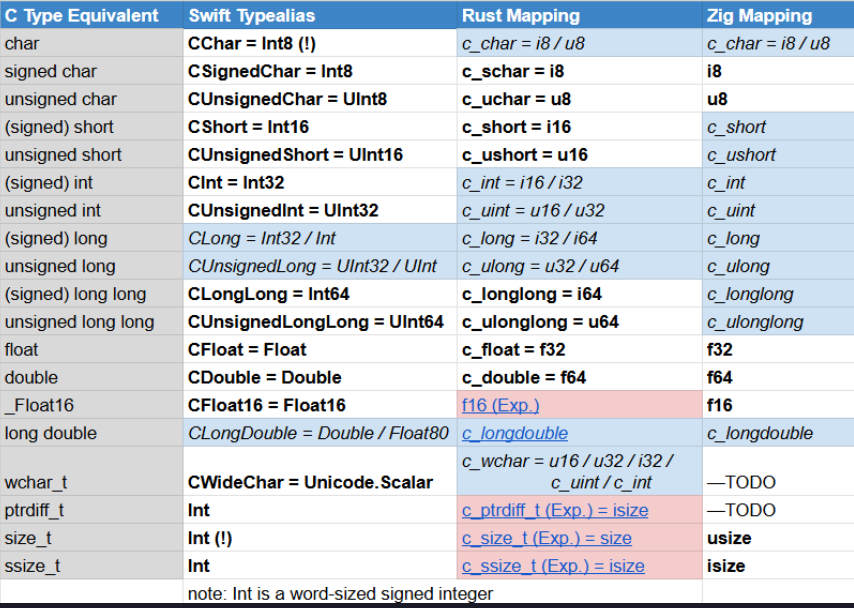
\includegraphics[width=\textwidth]{attachments/type comparison.png}
    \vspace{1em} % Add some space between image and sources/footnotes
    \footnotesize {
        Sources:
        \href{https://github.com/swiftlang/swift/blob/main/docs/HowSwiftImportsCAPIs.md#fundamental-types}{Swift1}, 
        \href{https://github.com/swiftlang/swift/blob/main/include/swift/ClangImporter/BuiltinMappedTypes.def}{Swift2}, 
        \href{https://github.com/rust-lang/rust/blob/master/library/core/src/ffi/primitives.rs}{Rust}, 
        \href{https://ziglang.org/documentation/0.14.1/#toc-Primitive-Types}{Zig} (todo make them citations)
    }

    \label{tab:type_mapping}    
\end{table}




On the other hand, Rust, Zig -- and also Hylo -- aim to support diverse platforms, including various embedded and mobile architectures, where C integer sizes may be defined differently. Rust and Zig introduced type aliases like \texttt{c\_long} that are aliasing fixed-sized types depending on the platform. \autoref{tab:type_mapping} presents a comparison of numeric type mapping in Swift, Rust, Zig and Muon. 



In Hylo, we propose a conservative approach by default, --similar to Zig-- but with a novel addition: instead of type aliases, we use distinct types for the C standard types which cannot be implicitly converted to Hylo's fixed-width integers. If type aliases were used, C's imported integer types may accidentally match fixed integer types, in which case the interoperability would be fragile when compiling for a different platform. Instead, Hylo should require explicit conversions whenever needed that clearly express the intent of the programmer. We have identified 3 types of necessary conversions:
\begin{itemize}
    \item \textbf{trap on loss:} when the conversion is narrowing, we insert a runtime assertion that ensures that the particular input can be represented in the target type. We provide this as the default conversion, e.g. \texttt{Int32(c\_value)}. When the conversion is non-narrowing, the assertion is not needed, and a zero-extend/sign-extend operation is performed based on signedness. Additionally, this default and recommended trapping behavior could be disabled with a compiler flag to sacrifice safety for maximal runtime performance.
    \item \textbf{truncate if needed:} when the represented value's meaning allows, we can silently drop the most significant bits that don't fit the target type. Note, due to two's complement representation, values that fit in the target type will preserve their sign. This may be spelled as \texttt{Int32(truncating\_if\_needed: c\_value)}
    \item \textbf{don't narrow:} when performance is critical but we also want a compile-time guarantee that a conversion is lossless on the target platform, we can use this conversion. \texttt{Int32(non\_narrowing: c\_value)} is a conditionally enabled conversion that is only available when the conversion would be lossless.
\end{itemize}
Using these explicit conversions ensures that we explicitly capture the programmer's intent and the code remains maximally portable. The viability of the approach was validated by implementing a code generator that produces the conversion function code for the standard library, detailed in Section 5.

However, writing all these conversions by hand may be very inconvenient, especially when we have solid assumptions about the target platform. E.g. when writing a wrapper around the LLVM compiler, we know that it will only be used on modern desktop platforms, where we can define many of the mappings like Swift or Muon did. Therefore, we allow making project-specific explicit assumptions about the target platforms, such as \texttt{c\_short} is 16-bit. These assumptions are checked for all the specified target platforms before compilation, so there are no risks introduced.

In addition, if a Hylo project generally uses the \texttt{Int} or \texttt{Int32} type for indices, it may specify to translate all \texttt{size\_t} function parameters to the expected types in all or some methods. Unless the bit-width is the same, this may involve truncation, which could be configured to trap on overflow or an error \emph{before} compilation. When a runtime conversion is needed, the original C function is not exposed to our Hylo code, instead a new wrapper function calling it and performing the necessary checks is exposed.

\vspace{1em} % Add some space
\textit{TODO:}
\begin{itemize}
    \item write about floats, complex\&imaginary number types, bool, and some other platform-defined types such as wchar\_t and size\_t.
\end{itemize}

Other primitive types are mapped as follows:
\begin{itemize}
    \item C's \texttt{\_Bool} is mapped to Hylo's \texttt{Bool}.
    \item C's \texttt{wchar\_t} for wide characters is mapped to a distinct \texttt{CWideChar} type in Hylo.
\end{itemize}

\subsubsection{Floating Point Types}
Real floating point numbers: \texttt{float}, \texttt{double}, \texttt{long double}
\begin{itemize}
    \item map them to \texttt{CFloat}, \texttt{CDouble}, \texttt{CLongDouble}
    \item The C standard does not mandate conformance to the ISO/IEC 60559 standard, but for now Hylo can mandate it. 
    \item conversions to Hylo's types:
        \begin{itemize}
            \item widening: preserving values
            \item narrowing: rounding, overflow to +-infinity or underflow to 0
            \item types of conversion functions
                \begin{itemize}
                    \item \texttt{init(non\_narrowing: other)}
                \end{itemize}
        \end{itemize}
    \item for now, import them as \texttt{Float}, \texttt{Double} in Hylo, require conformance of C compiler to the ISO/IEC 60559 standard (\texttt{\_\_STDC\_IEC\_60559\_BFP\_\_}). Later, we may allow importing them as \texttt{CFloat}, but keep supporting importing as \texttt{Float}/\texttt{Double}, inserting conversion functions on platform where necessary. \textit{todo} see which platforms have different float representations if any
\end{itemize}
Optional standard features (compilers are not required to implement them for standard compliance): complex numbers (since C99), decimal floating point numbers (since C23) -- these could be implemented without an issue in libraries. Complex numbers have specific hardware support for some operations, so the set of built-ins may need to be extended. They are not yet a priority.

\subsection{Composite Types}

\begin{itemize}
    \item \textbf{Structs:} C \texttt{struct}s are mapped to Hylo \texttt{struct}s with a \texttt{@CLayout} attribute, which instructs the compiler to use the target platform's C-compatible memory layout (including padding, alignment and correct offsets for bit-fields).
    \item \textbf{Unions:} TODO write
    \item \textbf{Arrays:} TODO write
    \item \textbf{Bitfields:} C bitfields have notoriously implementation-defined layout rules. To provide a safe and portable abstraction, bitfields are not exposed directly. Instead, they are imported as a private storage property of an appropriate integer size, and the interoperability tool generates safe getter and setter computed properties in Hylo that perform the necessary bit masking and shifting to access the individual fields.
\end{itemize}

\subsection{Pointer Types}

Pointers are central to C but are a primary source of memory safety issues. To bridge this gap, C pointers are mapped to Hylo's dedicated pointer types, which enforce safety rules:
\begin{itemize}
    \item A \texttt{const} C pointer (\texttt{const T*}) is mapped to Hylo's \texttt{Pointer<T>}, which provides read-only access.
    \item A mutable C pointer (\texttt{T*}) is mapped to Hylo's \texttt{PointerToMutable<T>}, which provides read-write access. Accessing memory through these pointers is an \texttt{unsafe} operation in Hylo.
    \item C function pointers are mapped to Hylo closure types with a \texttt{@convention(C)} attribute and an empty environment, which ensures that the correct calling convention is used when the function is called. \href{https://github.com/orgs/hylo-lang/discussions/1705}{relevant github discussion}
\end{itemize}

\subsection{Type Qualifiers}

C's type qualifiers are handled to preserve their semantics:
\begin{itemize}
    \item \texttt{const}: As described above, \texttt{const} affects the mutability of the resulting pointer or data type in Hylo.
    \item \texttt{volatile}, \texttt{restrict}, \texttt{\_Atomic}: These qualifiers signal special properties to the compiler. They are shall be represented in Hylo's type system to ensure that these semantics can be respected and passed on to the LLVM backend. Further research is necessary to see how to handle these properly, many interop technologies ignore them. (todo)   
\end{itemize}

\subsection{Customization and Ambiguous Mappings}

A core principle of our design is acknowledging that a single, direct mapping is often insufficient. Many C constructs are used to represent different semantic ideas. A prime example is the C \texttt{enum}. It can represent:
\begin{enumerate}
    \item A set of mutually exclusive cases \(\rightarrow\) translate to a Hylo enum for proper exhaustiveness checking
    \item A collection of independent bitflags \(\rightarrow\) translate to an \texttt{OptionSet} \cite{optionset} for easy combination and checking of binary flags.
    \item A simple group of named integer constants. \(\rightarrow\) translate to a Hylo namespace with constants.
\end{enumerate}
A rigid mapping to a single Hylo construct would be un-idiomatic in at least two of these cases. Therefore, our design proposes a system of \textbf{sensible defaults with user-customizable overrides.} By default, an \texttt{enum} might be imported as a struct of static constants, which is always safe. However, the developer can provide an annotation (e.g., in a separate configuration file or directly in the C header if they have ownership) to guide the mapping:

This principle of user-guided mapping extends to other areas, such as specifying that a C function returning an integer error code should be imported as a Hylo function that \texttt{throws}. This empowers developers to create bindings that are not only correct but also safe and highly idiomatic.